\documentclass[12pt]{article}
\usepackage[top = 3cm,bottom=3cm,left=2cm,right=2cm]{geometry}        
\geometry{letterpaper}
\usepackage[parfill]{parskip}  
\usepackage{graphicx}
\usepackage{amssymb}
\usepackage{epstopdf}
\usepackage{listings}
\usepackage{color}
\usepackage{amsmath}
\usepackage{tikz}
\usepackage{mathtools}
\usetikzlibrary{decorations.markings,arrows}
\usepackage{bm}
\usepackage{bbm}
\usepackage{hyperref}
 
 \begin{document}  
 
\baselineskip 2.7ex
\parskip 3.5ex

\pagestyle{myheadings}
\markright{\today \hfill Makeup Midterm Solutions \hfill}


%Equations/Entries
\newcommand{\beq}{\begin{equation}}
\newcommand{\bequo}{\begin{quotation}}
\newcommand{\beqa}{\begin{eqnarray}}
\newcommand{\eeq}{\end{equation}}
\newcommand{\leeq}[1]{\label{#1}\end{equation}}
\newcommand{\equo}{\end{quotation}}
\newcommand{\eeqa}{\end{eqnarray}}
\newcommand{\non}{\nonumber}
\newcommand{\mx}{\mbox}
\newcommand{\mxf}[1]{\mbox{\footnotesize{#1}}}
\newcommand{\lb}{\label}
\newcommand{\fr}[1]{(\ref{#1})}
\newtheorem{entry}{}[section]
\newcommand{\bent}[1]{\vspace*{-2cm}\hspace*{-1cm}\begin{entry}\lb{e{#1}}\rm}
\newcommand{\eent}{\end{entry}}
\newcommand{\fre}[1]{{\bf\ref{e{#1}}}}
\newcommand{\Emark}{$\sqcap\hspace{-2.7mm}\sqcup$}
\newcommand{\sEmark}{{\fns $\sqcap\hspace{-2.3mm}\sqcup$}}
\newcommand{\fn}{\footnote}


%Greek Letters
\renewcommand{\a}{\alpha}
\renewcommand{\b}{\beta}
\newcommand{\g}{\gamma}
\newcommand{\G}{\Gamma}
\renewcommand{\d}{\delta}
\renewcommand{\th}{\theta}
\renewcommand{\k}{\kappa}
\newcommand{\Th}{\Theta}
\newcommand{\D}{\Delta}
\newcommand{\e}{\epsilon}
\newcommand{\ep}{\varepsilon}
\newcommand{\s}{\sigma}
\renewcommand{\S}{\Sigma}
\newcommand{\w}{\omega}
\newcommand{\W}{\Omega}
\newcommand{\al}{\alpha}
\newcommand{\bet}{\beta}
\newcommand{\gam}{\gamma}
\newcommand{\lam}{\lambda}
\newcommand{\Lam}{\Lambda}
\newcommand{\eps}{\varepsilon}
\newcommand{\ichi}\sichi
\renewcommand{\ni}{\sni}
\renewcommand{\r}{\rho}
\renewcommand{\t}{\tau}
\newcommand{\ph}{\varphi}
\newcommand{\sichi}{{\mbox{{\footnotesize I}}}}
\newcommand{\sni}{{\mbox{{\footnotesize II}}}}

%color2010/6/9
\newcommand{\red}{\color{red}}
\newcommand{\blue}{\color{blue}}
\newcommand{\green}{\color{green}}
\definecolor{gray}{rgb}{0.5, 0.5, 0.5}
\newcommand{\gray}{\color{gray}}

%Derivatives
\newcommand{\pder}[2]{\frac{\partial {#1}}{\partial {#2}}}
\newcommand{\pdert}[2]{\frac{\partial^2 {#1}}{\partial {#2}^2}}
\newcommand{\fder}[2]{\frac{\delta {#1}}{\delta {#2}}}
\newcommand{\PDD}[3]{\left.\frac{\partial^{2}{#1}}{\partial{#2}^{2}}\right|_{#3}
}
\newcommand{\PD}[3]{\left.\frac{\partial{#1}}{\partial{#2}}\right|_{#3}}
\newcommand{\der}[2]{\frac{d {#1}}{d {#2}}}

\renewcommand{\deg}{^\circ}
\newcommand{\com}{{\bf [C] }}
\newcommand{\cend}{\Emark\[\]\vspace*{-1. cm}}
\newcommand{\x}{\times}

%My commands
\newcommand{\win}{\ddot\smile}
\newcommand{\lose}{\ddot\frown}
\newcommand{\avg}[1]{\left \langle #1 \right \rangle}
\newcommand{\E}[1]{\ensuremath{\times10^{#1}}}
\newcommand{\abs}[1]{\ensuremath{\left | #1 \right |}}
\newcommand{\paren}[1]{\left(#1\right)}
\newcommand{\recip}[1]{\frac{1}{#1}}
\newcommand{\ex}[1]{\mathbb{E}[#1]}
\newcommand{\bprob}[1]{\textbf{#1~---}}
\newcommand{\unitv}[1]{\ensuremath{\mathbf{\hat{e}}_{#1}}}
\newcommand{\goto}{\rightarrow}
\newcommand{\expct}[1]{\mathbb{E}[#1]}
\newcommand{\mtrx}[1]{\begin{matrix}#1\end{matrix}}
\newcommand{\pmtrx}[1]{\paren{\begin{matrix}#1\end{matrix}}}
\newcommand{\cosp}[1]{\cos{\paren{#1}}}
\newcommand{\sinp}[1]{\sin{\paren{#1}}}
\newcommand{\tanp}[1]{\tan{\paren{#1}}}
\newcommand{\half}[1]{\frac{#1}{2}}
\newcommand{\ham}{\mathcal{H}}
\newcommand{\tr}{\mathrm{Tr}}
\newcommand{\bv}[1]{\mathbf{#1}}
\newcommand{\Der}[2]{\frac{d#1}{d#2}}
\renewcommand{\Dot}[2]{\ensuremath{\bv{#1}\cdot\bv{#2}}}
\newcommand{\Cross}[2]{\ensuremath{\bv{#1}\times\bv{#2}}}
\newcommand{\del}{\ensuremath{\partial}}
\newcommand{\R}{\ensuremath{\bv{r-r'}}}
\newcommand{\aR}{\ensuremath{\abs{\R}}}
\newcommand{\br}{\ensuremath{\bv{r}}}
\newcommand{\impl}{\ensuremath{\quad \Rightarrow \quad}}
\renewcommand{\div}[1]{\nabla \cdot \bv{#1}}
\newcommand{\curl}[1]{\nabla \times \bv{#1}}
\newcommand{\lapl}{\nabla^2}
\newcommand{\vint}{\int d^3r}
\newcommand{\oocs}{\recip{c^2}}
\newcommand{\mnfp}[1]{\frac{\mu_0 #1}{4\pi}}
\renewcommand{\iiint}{\int_{-\infty}^{\infty}}
\newcommand{\tpi}[1]{\paren{2\pi}^{#1}}
\newcommand{\ootpi}[1]{\recip{\paren{2\pi}^{#1}}}
\newcommand{\Sig}{\bm{\s}}
\renewcommand{\dag}{^\dagger}

%%%%%%%%%%%%%%%%%%%%%%%

\bprob{1a} The one-site partition function is:
\[ Q_1 = 1+ e^{-\b \ep}.\]
All the sites are independent, so this is the only partition function that really matters. The probabilities are then
\[ p_0 = \recip{1+e^{-\b \ep}},\qquad p_\ep = \frac{e^{-\b \ep}}{1+e^{-\b \ep}}.\]
\begin{figure}[h]
\centering
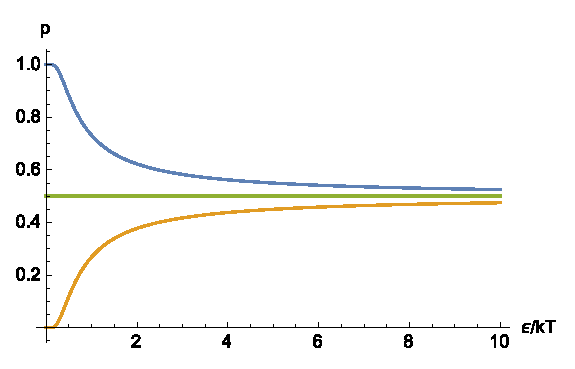
\includegraphics[scale=1.0]{probabilities_midterm.eps}
\caption{The blue curve is the probability of occupying the ground state, the yellow curve is the probability of occupying the excited state. The line $p=1/2$ is drawn for reference.}
\end{figure}

\bprob{1b} At $T=0$, there is no energy in the system and there should be 0 systems in the excited state (and all in the ground state). At infinite temperature, each state is equally likely, so the probabilities limit to $1/2$ for both states.

\bprob{1c} There are $\w$ states that have energy 0, now, so the partition function is
\[ Q_1 = 1 + 1 + 1 \ldots + 1 + e^{-\b\ep} = \w + e^{-\b \ep}.\]
The probability of having energy 0 or energy $\ep$ is
\[ p_0 = \frac{\w}{\w+e^{-\b\ep}}, \qquad p_\ep = \frac{e^{-\b\ep}}{\w + e^{-\b \ep}}.\]

\bprob{1d} At $T=0$, all of the systems should be in one of the $\w$ ground states, and none in the excited state. As $T\goto \infty$, we see that $e^{-\b\ep}\goto 1$, and
\[ p_0(T=\infty) = \frac{\w}{\w+1},\qquad p_\ep(T=\infty) = \recip{1+\w}.\]

\bprob{1e} The easiest way to see that the entropy is nonzero is to consider how many states each system has available at $T=0$. The systems can only explore their ground states, of which they have $\w$, so the entropy is
\[ S = k_B\log \w.\]
Or we can take
\[ \frac{S}{k_B} = \frac{\avg{E} - A}{k_BT}.\]
\[ \frac{S}{k_B} = -\b\pder{\log Q_1}{\b} + \log Q_1.\]
\[ \frac{S}{k_B} = \frac{\b\ep e^{-\b\ep}}{\w+e^{-\b\ep}} + \log\paren{\w+e^{-\b\ep}}.\]
As $\b\goto \infty$, the first term vanishes, and the second term just becomes $\log\w$.
\[ S \goto k_B \log\w.\]

\hrulefill

\bprob{2a} This problem doesn't require a Maxwell relation, just the cyclic identity:
\[ \PD{X}{Y}{Z} \PD{Y}{Z}{X} \PD{Z}{X}{Y} = -1.\]
Here, we want a relation with $T,B,$ and $S$:
\[ \PD{S}{B}{T}\PD{B}{T}{S}\PD{T}{S}{B} = -1.\]
\[ \paren{\PD{S}{B}{T}} \paren{ \PD BTS} \paren{\frac{T}{C_B}} = -1.\]
\[ \PD TBS = -\frac{T}{C_B}\PD SBT > 0.\]

\bprob{2b} We can use the result from part a and a Maxwell relation.
\[ \PD SBT = \PD MTB.\]
So we have
\[ \PD TBS = -\frac{T}{C_B}\PD MTB.\]
We can get $\PD MTB$ from the equation of state. Taking a derivative with respect to temperature:
\[ Mk_B + k_BT \PD MTB = N\PD BTB + J\PD MTB.\]
The term $\PD BTB = 0$, because we're holding $B$ constant, of course. So, rearranging, we have
\[ \PD MTB = \frac{-Mk_B}{k_BT-J}.\]
If we plug in $M = NB/(k_BT-J),$
\[ \PD MTB = \frac{-Nk_B B}{(k_BT-J)^2}.\]
Plugging this back in to $\PD TBS$,
\[ \PD TBS = \frac{Nk_BT B}{(k_BT-J)^2C_B}.\]
This is positive unless $k_BT = J$, where it is actually undefined. This equation of state is actually the equation of state of a ferromagnet in the limit of small $B$ and small $M$. $J$ is the strength of the coupling between magnetic moments, and when this energy becomes close to the order of $k_BT$, the system switches from one phase (paramagnetic) to another phase (ferromagnetic). This is similar to the phase transition in the Van der Waals equation that we'll be studying later.

\hrulefill

\bprob{3a} At constant $E,V,$ and $N$, this is the microcanonical ensemble, where all available microstates are equally likely, so we have
\[ p = \recip{\Omega(E,V,N)}.\]

\bprob{3b} The canonical partition function is defined as
\[ Q(N,V,T) = \sum_{\nu(N,V,E)} e^{-\b E_{\nu(N,V,E)}}.\]
Here, the sum over $\nu$ is restricted to microstates that have a constant volume, particle number, and energy. We can write this more naturally as
\[ Q(N,V,T) = \sum_E \Omega(E,V,N) e^{-\b E}.\]
This still sums over all the states of constant energy, volume, and particle number, but we're explicitly writing that we're summing over energies, not microstates, so we must include a factor that counts how many microstates have energy $E$. The probability of observing \emph{a} microstate with energy $E$ is
\[ p_{\nu(E)} = \frac{e^{-\b E}}{Q(N,V,T)}.\]
The probability of observing \textbf{any} microstate whose energy is $E$, that is, the probability of observing that the system has energy $E$ is
\[ p_E = \frac{\Omega(N,V,E)e^{-\b E}}{Q(N,V,T)}.\]
I accepted both answers, because the difference is very subtle.

\bprob{3c} We can write the grand canonical partition function as
\[ \Xi(\mu,V,T) = \sum_N\sum_E \Omega(E,V,N) e^{-\b E + \b N \mu} = \sum_N Q(N,V,T)e^{\b N \mu}.\]
The probability of observing \emph{a} microstate with energy $E$ and particle number $N$ is
\[ p_{\nu(E,N)} = \frac{e^{-\b E +\b N \mu}}{\Xi(\mu,V,T)}.\]
The probability of observing \textbf{any} microstate with energy $E$ and particle number $N$, that is, the probability of observing that the system has energy $E$ and particle number $N$ is
\[ p_{E,N} = \frac{\Omega(E,N,V)e^{-\b E + \b N \mu}}{\Xi(\mu,V,T)}.\]
Once again, I accepted either answer.

\bprob{3d} To transform from the constant-shape ensemble to the constant-alchemical potential ensemble, we perform a transformation that should look exactly like the grand canonical ensemble transformation, because $\a$ and $d\s$ have the same role as $\mu$ and $dN$ in the thermodynamic relation $dE = TdS - PdV + \mu dN + \a d\s$.
\[ \Theta(T,V,N,\a) = \sum_\s Q(T,V,N,\s) e^{\b \a \s}.\]
What this means is that we have to somehow specify the shape of our particles by some variable $\s$, then we have to find a way to sum over all possible values of $\s$. For example, for simplicity, we could look at two dimensions. The unit circle is defined by
\[ 1 = x^2 + y^2.\]
A diamond shape whose corners are $(\pm1,0)$ and $(0,\pm1)$ can be defined by
\[ 1 = \abs{x} + \abs{y}.\]
If we let
\[ 1 = \abs{x}^\s + \abs{y}^\s,\]
we can ramp $\s$ from 1 to 2 to go continuously from a diamond to a circle.
\begin{figure}[h]
\centering
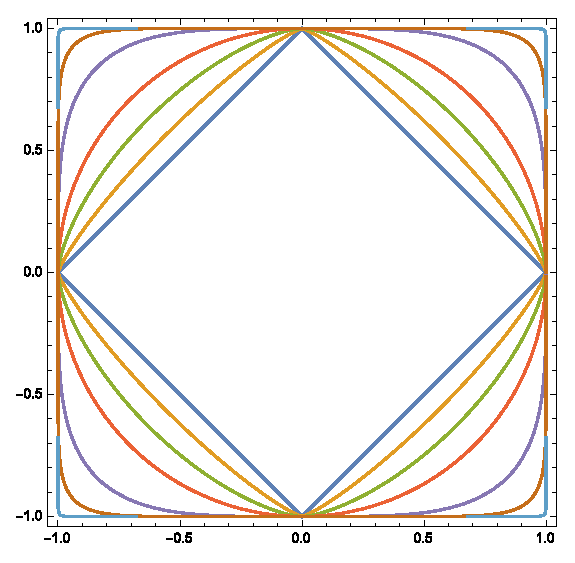
\includegraphics[scale=1.0]{shapes.eps}
\caption{The plot $1=\abs{x}^\s + \abs{y}^\s$ plotted for $\s = 1,1.2,1.5,2,4,10,100$. As $\s\goto \infty$, we have a square.}
\end{figure}
This is just an example of how we might perform a summation like this: if we allow $\s$ to take discrete values, we'd sum over those discrete values, and if it were continuous, we'd do an integration like we do when we do phase space integrals.

\hrulefill

\bprob{4a} The canonical partition function for one particle is
\[ Q_1 = \recip{h^2} \int d\bv p \int d\bv r \, e^{-\frac{\b p^2}{2m} + \half{1}\b m\w^2 r^2}.\]
The momentum integral we've done many times, so we just pick up two factors of the thermal wavelength:
\[ Q_1 = \recip{\lam^2} \int d\bv r \, e^{\half{1}\b m \w^2 r^2}.\]
Note that there is a positive sign in the exponent! This isn't a Gaussian integral, but it is actually very simple when we go to polar coordinates, the transformation of which was given on the back of the exam:
\[ Q_1 = \recip{\lam^2} \int_0^{2\pi}d\th \int_0^R rdr \, e^{\half{1} \b m \w^2 r^2}.\]
The angular integral gives $2\pi$, and we can define $u = \half{\b m \w^2}r^2$:
\[ Q_1 = \frac{2\pi}{\lam^2 \b m \w^2} \int_0^{\half{\b m \w^2 R^2}} du \, e^{u}.\]
\[ Q_1 = \frac{2\pi}{\lam^2\b m \w^2} \paren{e^{\half{\b m \w^2 R^2}} - 1}.\]
We can substitute in the volume (area, really, we're in two dimensions) with $R^2 = V/\pi$:
\[ Q_1 = \frac{2\pi}{\lam^2\b m \w^2} \paren{e^{\frac{\b m \w^2 V}{2\pi}} - 1}.\]
The total partition function is of course $Q = Q_1^N/N!$.

\bprob{4b} The energy is
\[ E = -\pder{\log Q}{\b} = -N \pder{\log Q_1}{\b}.\]
\[ E = N\pder{}{\b}\paren{ 2\log \lam + \log \b - \log \paren{e^{\frac{\b m \w^2 V}{2\pi}} - 1} }.\]
Remember $\lam \propto \sqrt{\b}$:
\[ E = Nk_BT + Nk_BT - \frac{N m \w^2 V}{2\pi} \frac{e^{\frac{\b m \w^2V}{2\pi}} }{e^{\frac{\b m \w^2V}{2\pi}}  - 1}.\]
\[ E = Nk_BT + Nk_BT - \frac{N m \w^2 V}{2\pi} \frac{1}{1-e^{-\frac{\b m \w^2V}{2\pi}} }.\]
The first term $Nk_BT$ is the ideal gas term, which comes from equipartition. The second and third term are corrections. We can check that they will go away in $\w\goto 0$ limit:
\[ E(\w\goto 0) \approx Nk_BT + Nk_BT - \frac{N m \w^2 V}{2\pi} \frac{1}{\frac{\b m \w^2V}{2\pi}}.\]
\[ E \approx Nk_BT.\]

\bprob{4c} The pressure is very similar to the energy:
\[ P = -\pder{A}{V} = Nk_BT\pder{\log Q_1}{V}.\]
\[ P = Nk_BT \pder{}{V} \log \paren{ e^{\frac{\b m \w^2 V}{2\pi}} -1 }.\]
\[ P = \frac{Nm \w^2}{2\pi}  \frac{1}{1-e^{-\frac{\b m \w^2V}{2\pi}} }.\]
In the limit of really high temperatures $\b\goto 0$,
\[ P \goto \frac{N m \w^2} {2\pi} \frac{1}{\frac{\b m \w^2V}{2\pi} }.\]
\[ P \goto \frac{Nk_BT}{V}.\]

\bprob{4d}  The pressure at very \emph{low} temperatures is more interesting. The exponential in the denominator goes to 0, and we get
\[ P = \frac{N m \w^2}{2\pi}.\]
We can think of this from a totally mechanical perspective: at extremely low temperatures, the lowest energy state has all the particles pinned against the side of the container by the centrifugal force. This force is $F = m \w^2 R$ per particle. The pressure is a force divided by an area (but here in two dimensions, we divided the force by a length), and the length here is $2\pi R$, the circumference of the container. There are $N$ particles, so we have
\[ P = \frac{ N F}{2\pi R} = \frac{N m \w^2}{2\pi}.\]




\end{document}
